\documentclass{article}
\usepackage[utf8]{inputenc}
\usepackage{tikz}
\usetikzlibrary{mindmap}

\begin{document}

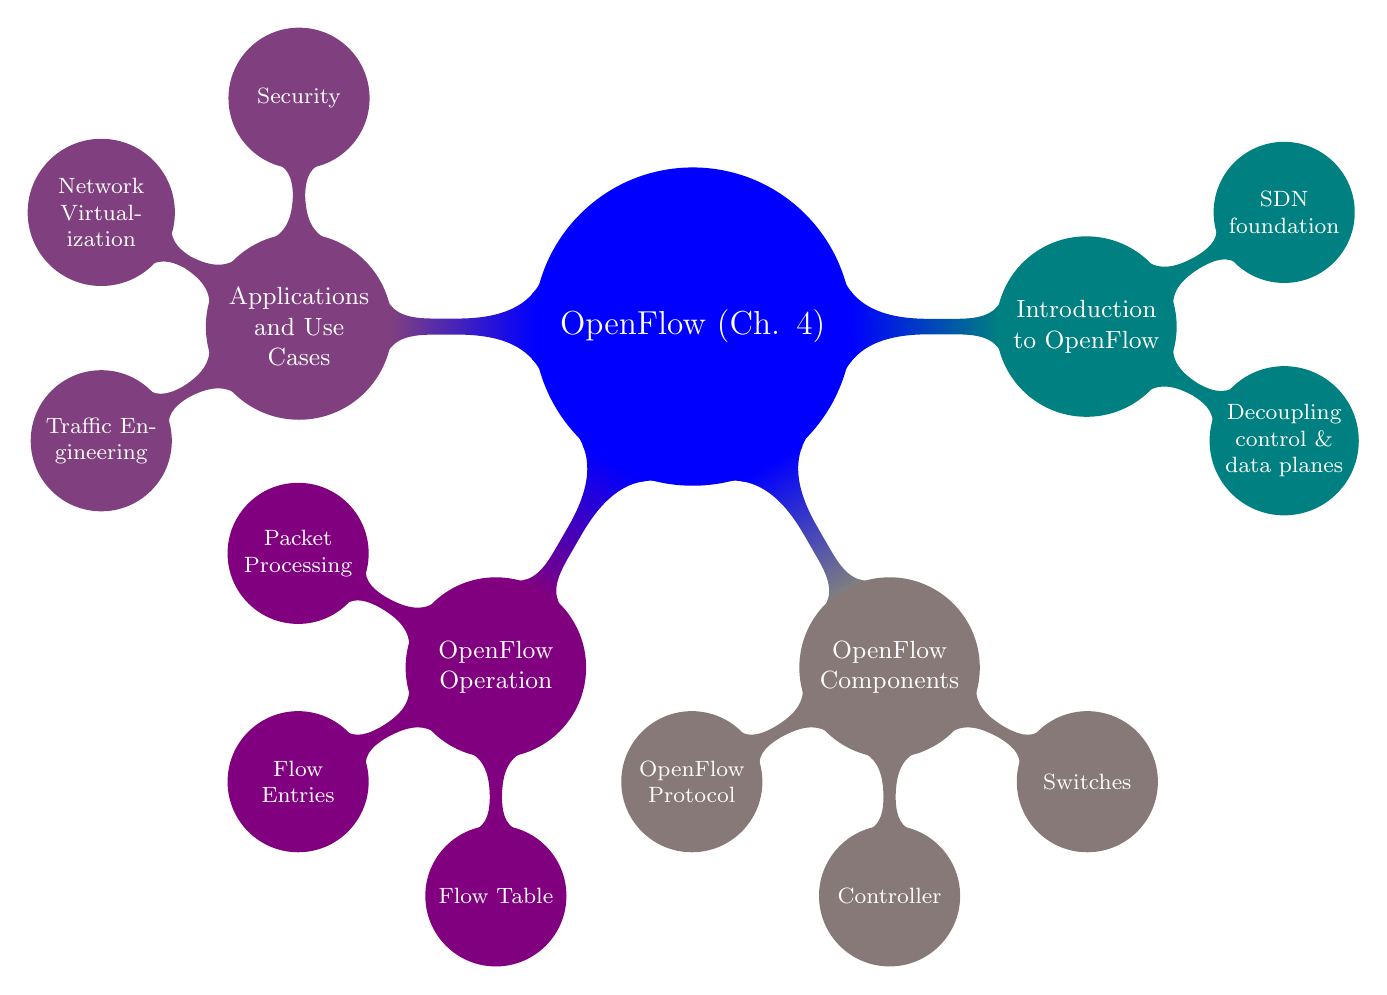
\begin{tikzpicture}
    \path[mindmap, concept color=blue, text=white]
        node[concept] {OpenFlow (Ch. 4)}
        [clockwise from=0]
        child[concept color=green!50!blue] {
            node[concept] {Introduction to OpenFlow}
            [clockwise from=30]
            child { node[concept] {SDN foundation} }
            child { node[concept] {Decoupling control \& data planes} }
        }
        child[concept color=yellow!50!blue] {
            node[concept] {OpenFlow Components}
            [clockwise from=-30]
            child { node[concept] {Switches} }
            child { node[concept] {Controller} }
            child { node[concept] {OpenFlow Protocol} }
        }
        child[concept color=red!50!blue] {
            node[concept] {OpenFlow Operation}
            [clockwise from=-90]
            child { node[concept] {Flow Table} }
            child { node[concept] {Flow Entries} }
            child { node[concept] {Packet Processing} }
        }
        child[concept color=orange!50!blue] {
            node[concept] {Applications and Use Cases}
            [clockwise from=-150]
            child { node[concept] {Traffic Engineering} }
            child { node[concept] {Network Virtualization} }
            child { node[concept] {Security} }
        };
\end{tikzpicture}

\end{document}
